%!TeX root=../tese.tex
%("dica" para o editor de texto: este arquivo é parte de um documento maior)
% para saber mais: https://tex.stackexchange.com/q/78101

\chapter{Algoritmo totalmente dinâmico para MSF}
\label{chapter:fully-MSF}

Neste capítulo, estudaremos o algoritmo totalmente dinâmico para MSF, o qual chamaremos de \textbf{MSF dinâmica}. Como este algoritmo não será implementado em nosso estudo, apresentaremos apenas a ideia por trás dele, de como podemos manter o peso mínimo de uma MSF de um grafo $G$ que suporte adição e remoção de arestas. Inicialmente, será descrito o funcionamento das \textbf{top trees}, estruturas de dados que serão usadas para construir a MSF dinâmica. Estas estruturas estão descritas na Seção~2.2 do artigo de Holm, de Lichtenberg e Thorup~\cite{jacob_holm}.

\section{Top trees}

A construção de uma top tree é baseada em um par ($T$, $\partial T$), onde $T$ é uma árvore e $\partial T$ é um conjunto que contém no máximo dois vértices de $T$, que são chamados vértices da fronteira (\textit{external boundary vertices}), como se pode ver na Figura~\ref{fig:top-tree-pair-representation}.

\begin{figure}[H]
    \centering
    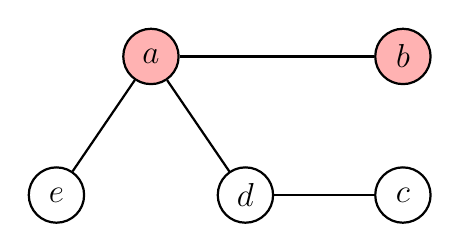
\begin{tikzpicture}
        [scale=0.8, node/.style={circle,draw,minimum size=2em, thick, font=\large},
        edge/.style={thick, black},
        reserve/.style={red, thick},
        removed/.style={black, thick, dashed}, 
        inner sep=0pt]

        \node[node, fill=red!30] (a) at (0,1.5) {$a$};
        \node[node, fill=red!30] (b) at (4,1.5) {$b$};
        \node[node] (c) at (4,-0.7) {$c$};
        \node[node] (d) at (1.5,-0.7) {$d$};
        \node[node] (e) at (-1.5,-0.7) {$e$};

        \draw[edge] (a) -- (b) node[midway, above] {};
        \draw[edge] (c) -- (d) node[midway, above] {};
        \draw[edge] (d) -- (a) node[midway, above] {};
        \draw[edge] (a) -- (e) node[midway, above] {};

    \end{tikzpicture}
    \caption{Representação de uma árvore $T$ de $5$ vértices. Os vértices pintados em vermelho são vértices da fronteira de $T$, ou seja, formam o conjunto $\partial T$.}
    \label{fig:top-tree-pair-representation}
\end{figure}

Assim, dado ($T$, $\partial T$), qualquer subárvore $S$ de $T$ tem um conjunto $\partial_{(T, \partial T)}S$ de vértices da fronteira, que são vértices de $S$ que estão ou em $\partial T$ ou são incidentes a uma aresta de $T$ saindo de $S$, como se pode ver no exemplo da Figura~\ref{fig:top-tree-subtree-option1}.

\begin{figure}[H]
    \centering
    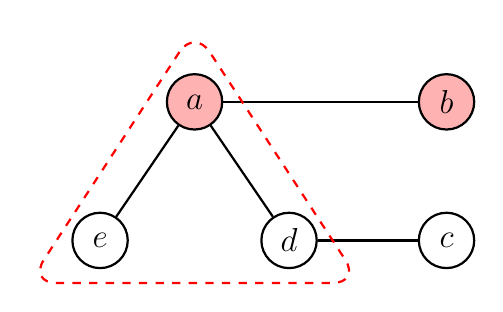
\begin{tikzpicture}
        [scale=0.8, node/.style={circle,draw,minimum size=2em, thick, font=\large},
        edge/.style={thick, black},
        reserve/.style={red, thick},
        removed/.style={black, thick, dashed}, 
        inner sep=0pt]

        \node[node, fill=red!30] (a) at (0,1.5) {$a$};
        \node[node, fill=red!30] (b) at (4,1.5) {$b$};
        \node[node] (c) at (4,-0.7) {$c$};
        \node[node] (d) at (1.5,-0.7) {$d$};
        \node[node] (e) at (-1.5,-0.7) {$e$};

        \draw[edge] (a) -- (b) node[midway, above] {};
        \draw[edge] (c) -- (d) node[midway, above] {};
        \draw[edge] (d) -- (a) node[midway, above] {};
        \draw[edge] (a) -- (e) node[midway, above] {};
        
        % P1: Top Vertex (above node 'a')
        \coordinate (P1) at ([yshift=20pt]a.north); 
        
        % P2: Bottom-Left Vertex (left of 'e' and slightly below it, using calc for precision)
        \coordinate (P2) at ([xshift=-23pt, yshift=-10pt]e.south west);
        
        % P3: Bottom-Right Vertex (right of 'd' and slightly below it, using calc for precision)
        \coordinate (P3) at ([xshift=23pt, yshift=-10pt]d.south east);

        % --- Draw the Dashed Triangular Outline ---
        
        % Connect the invisible coordinates with rounded corners
        \draw[dashed, thick, red, rounded corners=10pt] 
            (P1) -- (P2) -- (P3) -- cycle;

        % \draw[dashed, thick, red] (e) -- (a) -- (d) -- cycle;
    \end{tikzpicture}
    \caption{Representação de uma árvore $T$ de $5$ vértices. Os vértices pintados em vermelho são vértices da fronteira de $T$, ou seja, formam o conjunto $\partial T$. O triângulo tracejado representa a subárvore $S$ contendo os vértices $a$, $e$ e $d$ e as arestas $ae$ e $ad$. Neste exemplo, note que os vértices da fronteira de $S$ são $a$ e $d$.}
    \label{fig:top-tree-subtree-option1}
\end{figure}